\documentclass[10.5pt,notitlepage]{article}
\usepackage[utf8]{inputenc}
\usepackage{amsthm}
\usepackage{amsmath}
\usepackage{amsfonts}
\usepackage{mathtools}
\usepackage{amsmath,amssymb}       
\usepackage{enumitem}   
\usepackage{enumerate}
\usepackage{verbatim} 
\usepackage{bbm}
\usepackage{hyperref}
\usepackage{booktabs}
\renewcommand{\qedsymbol}{$\blacksquare$}
\usepackage{makecell}
\usepackage[spanish]{babel}
\decimalpoint
\usepackage[letterpaper]{geometry}
\usepackage{mathrsfs}
\newenvironment{solucion}
  {\begin{proof}[Solución]}
  {\end{proof}}
\pagestyle{plain}
\usepackage{pdflscape}
\usepackage[table, dvipsnames]{xcolor}
\usepackage{longtable}
\usepackage{tikz}
\def\checkmark{\tikz\fill[scale=0.4](0,.35) -- (.25,0) -- (1,.7) -- (.25,.15) -- cycle;} 
\usepackage[bottom]{footmisc}
\usepackage{hyperref}
\usepackage{float}
\usepackage[utf8]{inputenc}
\usepackage{bbm}
\usepackage[backend=biber,style=apa]{biblatex}
\usepackage{csquotes}
\DeclareLanguageMapping{spanish}{spanish-apa}
\urlstyle{same}
\addbibresource{refer.bib}
\usepackage{etoolbox}
\patchcmd{\thebibliography}{\section*{\refname}}{}{}{}
\usepackage{placeins}
\newcommand{\pp}{\mathbb{P}}
\newcommand{\BB}{\mathcal{B}}
\newcommand{\RR}{\mathbb{R}}
\newcommand{\Ff}{\mathcal{F}}
\newcommand{\Jj}{\mathcal{J}}
\newcommand{\Cc}{\mathcal{C}}
\newcommand{\oo}{\varnothing}
\newcommand{\ee}{\varepsilon}
\newcommand{\EE}{\mathbb{E}}
\newcommand{\NN}{\mathbb{N}}
\newcommand{\PP}{\mathcal{P}}
\newcommand{\LL}{\mathrm{L}}
\newcommand{\XX}{\mathbf{X}}
\newcommand{\xx}{\mathbf{x}}
\DeclareMathOperator{\Tr}{Tr}
\newcommand{\abs}[1]{\left\lvert #1 \right\rvert}
\newcommand{\norm}[1]{\left\| #1 \right\|}
\newcommand{\inner}[1]{\left\langle #1 \right\rangle}
\newcommand{\corch}[1]{\left[ #1 \right]}
\newcommand{\kis}[1]{\left\{ #1 \right\}}
\newcommand{\pare}[1]{\left( #1 \right)}

\theoremstyle{plain}

\newtheorem{thm}{Teorema}[section] % reset theorem numbering for each chapter
\newtheorem{defn}[thm]{Definición} % definition numbers are dependent on theorem numbers
\newtheorem{lem}[thm]{Lema} % same for example numbers
\newtheorem{remarkex}{Observación}
\newenvironment{rem}
  {\pushQED{\qed}\renewcommand{\qedsymbol}{$\triangle$}\remarkex}
  {\popQED\endremarkex}

\usepackage{geometry}
\usepackage{mathtools}
\usepackage{enumitem}
\usepackage{framed}
\usepackage{amsthm}
\usepackage{thmtools}
\usepackage{etoolbox}
\usepackage{fancybox}

\newenvironment{myleftbar}{%
\def\FrameCommand{\hspace{0.6em}\vrule width 2pt\hspace{0.6em}}%
\MakeFramed{\advance\hsize-\width \FrameRestore}}%
{\endMakeFramed}
\declaretheoremstyle[
spaceabove=6pt,
spacebelow=6pt
headfont=\normalfont\bfseries,
headpunct={} ,
headformat={\cornersize*{2pt}\ovalbox{\NAME~\NUMBER\ifstrequal{\NOTE}{}{\relax}{\NOTE}:}},
bodyfont=\normalfont,
]{exobreak}

\declaretheorem[style=exobreak, name=Ejercicio,%
postheadhook=\leavevmode\myleftbar, %
prefoothook = \endmyleftbar]{exo}
\usepackage{graphicx}
\graphicspath{ {images/} }
\title{Tarea 8: Modelos Estadísticos I.}

\author{Rojas Gutiérrez Rodolfo Emmanuel}

\begin{document}

\maketitle

\setcounter{exo}{0}
\begin{exo}\label{Ej.1}
Considere una muestra aleatoria \(Y_1, \hdots, Y_{N}\) con distribución exponencial
\[
f(y_i | \theta_i) = \theta_i\exp\kis{-\theta_i y_i }.
\]
Obtenga la deviance comparando el modelo máximal con diferentes valores de \(\theta_i\) para cada \(Y_i\) con el modelo con \(\theta_i = \theta\) para cada \(i \in \kis{1, \hdots, N}\).
\end{exo} 
\begin{solucion}
Primeramente, observe que para \(i \in \kis{1, \hdots, n}\) se tiene que
\begin{align*}
  f(y_i|\theta_i) &= \exp\kis{\ln(\theta_i)}\exp\kis{-\theta_i y_i}  \\
  &= \exp\kis{-\theta_i y_i + \ln(\theta_i)}. 
\end{align*}
Defina \(\phi = 1,\ \omega_i = 1,\ k(\theta_i) = -\ln(\theta_i)\) e \( c(y_i, \phi) = 0\), entonces, la densidad de la distribución exponencial con parámetro de forma \(\theta_i\), puede expresarse como:
\begin{equation*}
   f(y_i|\theta_i) =\exp\kis{\frac{y_i(-\theta_i) - k(\theta_i)}{\phi/\omega_i}+c(y_i, \phi ) } 
\end{equation*}
Por lo que, la distribución exponencial con parametro de forma \(\theta_i\) es un miembro de la familia exponencial de modelos de dispersión, con parámetro canónico \(\theta_i\). Luego, denote por \(\mathbf{y} = (y_1, \hdots,y_N)\) a la muestra aleatoria observada de las \(Y_i\) y note que la log-verosimilitud para la misma, esta dada por 
\begin{align}\label{3.1}
      l(\theta_1, \hdots,\theta_N|\mathbf{y}) &= \sum_{j=1}^{N}\corch{\frac{y_j(-\theta_j) - k(\theta_j)}{\phi/\omega_i}+c(y_j, \phi )} \nonumber\\ 
      &= \sum_{k=1}^{N}\corch{y_j(-\theta_j) + \ln(\theta_i)},
\end{align}
De este modo, para el modelo saturado suponiendo un parámetro distinto para cada \(Y_i\), obtenemos las siguientes ecuaciones Score a partir de la log-verosimilitud en \eqref{3.1} 
\begin{equation*}
    0= \frac{\partial l(\theta_1, \hdots,\theta_N|\mathbf{y})}{ \partial \theta_j} = -y_i + \frac{1}{\theta_i},\  i \in \kis{1, \hdots, N}.
\end{equation*}
Resolviendo el sistema de ecuaciones Score anterior, se obtiene la siguiente estimación por máxima verosimilitud para el parámetro natural \(\theta_i\): 
\begin{equation}\label{max}
  \tilde{\theta}_i = \frac{1}{y_i},\ i \in \kis{1, \hdots, N}.  
\end{equation}

Por último, si suponemos un modelo en el que \(\theta_i = \theta >0\) para cada \(i \in \kis{1, \hdots, N}\), entonces, la log-verosimilitud en \eqref{3.1} se simplifica de la siguiente forma 
\[
l(\theta|\mathbf{y}) =  \sum_{k=1}^{N}\corch{y_i(-\theta) + \ln(\theta)},
\]
y por el curso de Inferencia Estadística I, sabemos que la log-verosimilitud anterior se maximiza en 
\begin{equation}\label{int}
    \hat{\theta}_i = \hat{\theta} = 1/\overline{y} \text{ con } i \in \kis{1, \hdots, N}.
\end{equation}
Así, la Deviance para el modelo de interés \(\theta_i = \theta\) para cada \(i \in \kis{1, \hdots, N}\), queda dada por 
\begin{equation*}
    D = 2\sum_{i = 1}^{N}\omega_i\corch{y_i(\tilde{\theta}_i - \hat{\theta}_i) -(k(\tilde{\theta}_i) + k(\hat{\theta}_i))},
\end{equation*}
donde \(\hat{\theta}_i\) y \(\tilde{\theta}_i\) con \(i\in \kis{1, \hdots, N}\) como fueron dados en \eqref{max} y \eqref{int}. Por último, recordando que \(\omega_i = 1\) para cada \(i \in \kis{1,\hdots, N}\) y que \(k(\theta) = -\ln(\theta)\), se obtiene la siguiente igualdad para la deviance 
\begin{align*}
      D &= 2\sum_{i = 1}^{N}\corch{y_i\pare{\frac{1}{y_i} - \frac{1}{\overline{y}}}+ \ln\pare{\frac{1}{\overline{y}}} - \ln\pare{\frac{1}{y_i}}}= 2\sum_{i = 1}^{N}\corch{1 - \ln\pare{\frac{y_i}{\overline{y}}} - \frac{y_i}{\overline{y}}}\\ 
      &=  2N + -2\sum_{i = 1}^{N}\corch{\ln\pare{\frac{y_i}{\overline{y}}}} - \frac{2N \overline{y}}{\overline{y}} = -2\sum_{i = 1}^{N}\corch{\ln\pare{\frac{y_i}{\overline{y}}}},
\end{align*}
es decir 
\[
D = -2\sum_{i = 1}^{N}\corch{\ln\pare{\frac{y_i}{\overline{y}}}}.
\]
Finalmente, bajo la hipótesis nula \(\mathcal{H}_0: \theta_i = \theta\) para cada \(i\in \kis{1,\hdots,N}\) se tiene que 
\[
D \sim \chi_{(N-1)}^{2}, \text{ de manera aproximada.}
\]
Por lo que, si \(\chi_{N-1, 1 - \alpha}^{2}\) denota al cuantil \(1- \alpha\) de una distribución Ji-cuadrada con \(N-1\) grados de libertad, rechazariamos dicha hipotesis en caso de que 
\[
D = -2\sum_{i = 1}^{N}\corch{\ln\pare{\frac{y_i}{\overline{y}}}}\geq \chi_{N-1, 1 - \alpha}^{2}.
\]
\end{solucion}

\begin{exo}\label{Ej.2}
Sea \(l(b_{\min})\) el valor máximo de la función de logverosimilitud para el modelo minimal con predictor lineal \(x'\beta = \beta_1\) y sea lineal \(x'\beta = \beta_1 + \beta_2 x_1 + \hdots \beta_p x_{p}\)
\begin{itemize}
    \item[a)] Pruebe que la estadística ji-cuadrada es 
    \[
    C = 2\corch{l(b) - l(b_{\min})} = D_0 - D_1, 
    \]
    donde \(D_0\) es la deviance para el modelo minimal y \(D_1\) para el modelo más general. 
    \item[b)] Deducir que si \(\beta_2 = \beta_3 = \hdots = \beta_p = 0\) entonces \(C\) tiene la distribución Ji-cuadrada central \(p-1\) grados de libertad.
\end{itemize}
\end{exo} 
\begin{solucion}
Primeramente, suponga que se cuenta con \(N\) observaciones, que \(1< p < N\) y denote por \(l(b)\) al valor máximo de la log-verosimilitud para el modelo con predictor lineal \(x'\beta =\beta_1 + \beta_2 x_1 + \hdots \beta_p x_{p}\). La deviance para el modelo minimal, se definió como la deviance nula y se sabe que esta dada por
\[
D_{0} = 2\corch{l(b_{\max}) - l(b_{\min})}, 
\]
donde, \(l(b_{\max})\) denota al valor máximo de la verosimilitud para el modelo saturado. Por otro lado, la deviance para el modelo más general, con predictor lineal \(x'\beta =\beta_1 + \beta_2 x_1 + \hdots \beta_p x_{p-1}\), esta dada por 
\[
D_{1} =  2\corch{l(b_{\max}) - l(b)}. 
\]
Asi, de lo visto en clase se sabe que bajo la hipótesis nula \(\mathcal{H}_0: \beta_{2} = \hdots = \beta_{p} = 0\), se tiene que \(D_0 \sim \chi^{2}_{N-1}\) y que \(D_{1} \sim \chi_{N-p}^{2}\), y por ende se tiene que
 
\[
  D_{0} - D_{1} \sim \chi^{2}_{(N-1)-(N-p)} = \chi^{2}_{p-1}.
\]
Note, que la anterior es la estadística ji-cuadrada que compara el modelo con \(p\) parámetros, contra el modelo minimal, qué es o eso creo la estadística \(Ji\) cuadrada solicitada, el resultado se sigue ahora de notar que 
\[
  D_{0} - D_{1} =  2\corch{l(b_{\max}) - l(b_{\min})} - 2\corch{l(b_{\max}) - l(b)} =  2\corch{l(b) - l(b_{\min})}.
\]
\end{solucion}


\begin{exo}\label{Ej.3}
El número de muertes por leucemia y otros tipos de cáncer entre supervivientes de la bomba atómica de Hiroshima se muestran en la Tabla en la figura \ref{fig:my_label}, clasificados por la dosis de radiación recibida. Los datos se refieren a muertes durante el periodo 1950-1959, entre supervivientes cuyas edades estaban entre 25 y 64 años en 1950. Obtener un modelo adecuado para describir la relación dosis –respuesta entre la radiación y las tasas de mortalidad proporcionales para leucemia. 
\end{exo} 
\begin{figure}[htb]
    \centering
    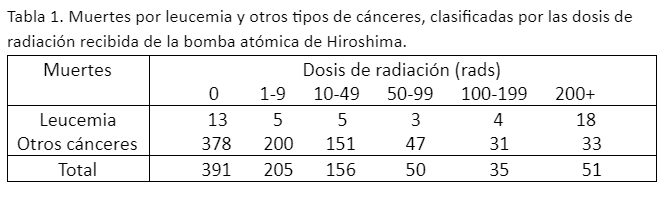
\includegraphics[scale = 0.8]{Im1.png}
    \caption{Datos: Ejercicio 3}
    \label{fig:my_label}
\end{figure}
\begin{solucion}
Primeramente, denote por \(y = \begin{pmatrix}13 &5&5&3&4&18 \end{pmatrix}'\) al vector columna de observaciones de casos de Leucemia por grupo de exposición y por \(T = \begin{pmatrix} 391 &205 &156& 50 &35& 51 \end{pmatrix}'\) al vector columna con el total de individuos por grupo de exposición, entonces, el vector columna \(P\) con entradas:
\begin{equation*}
    P_i = y_i / T_i, \ i \in \kis{1, \hdots, 6},
\end{equation*}
nos da la proporción de individuos que murieron en cada grupo a causa de la leucemia, dado que fallecieron por algún tipo de cáncer. Utilizando dicho vector, se construyo la gráfica en la figura \ref{figIm1}.
\begin{figure}[htb]
    \centering
    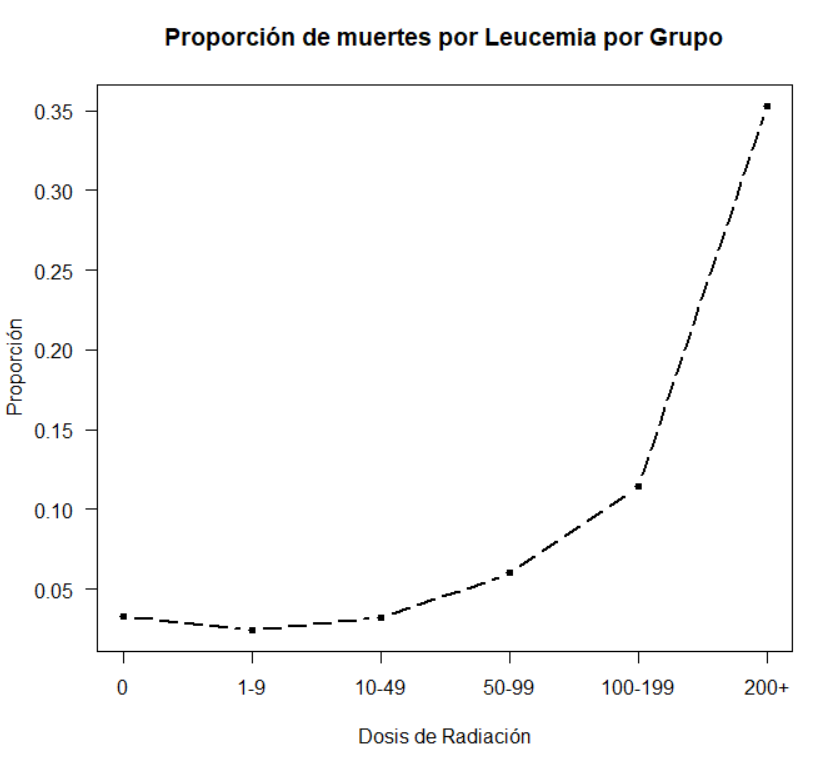
\includegraphics[scale= 0.7]{Im1Ej4.png}
    \caption{Proporción del número de muertes por leucemia, por grado de exposición a la radiación al que estuvieron expuestos los individuos.}
    \label{figIm1}
\end{figure}
En dicha gráfica, podemos notar que existe una relación casi creciente entre la proporción de muertes por leucemia, respecto a muertes por otros tipos de cáncer, y la dosis de radiación a la que estuvieron expuestos los distintos individuos en cada grupo. Ahora, piense a la proporción de muertes por leucemia y no por otro tipo de cáncer por cada nivel de radiación, como una estimación de la probabilidad de morir por Leucemía y no por otro cáncer, dado que la causa de muerte fue cáncer y que se estuvo expuesto a un cierto nivel de radiación, bajo este contexto, se propone modelar la relación dosis-respuesta entre la dosis de radiación y las tasas de mortalidad para leucemia, de la siguiente manera. Sea \(x = (0,1,10,50,100,200)'\) el vector columna con los extremos izquierdos de cada uno de los intervalos de dosis de radiación, a las que pertenecen las distintas proporciones de muertes por leucemia, se propone un modelo lineal generalizado de la familia binomial, para modelar la probabilidad de morir por leucemia dado que la causa de muerte fue cáncer y dado que se estuvo expuesto a cierto nivel de radiación, es decir un modelo de la forma:
\begin{equation}\label{glm1}
   g(\pi_i) = \beta_0 + \beta_1 x_i, \ i\in \kis{1, \hdots,6},  
\end{equation}
donde \(g\) es una función liga, la cual se elegirá entre las tres más utilizadas para este tipo de modelos: la logit, la probit o la logaritmo complementaria y \(\pi_i\) con \(i \in \kis{1, \hdots, 6}\) denota a la probabilidad de morir por leucemia en lugar de por otro cáncer, dado que la causa de muerte fue cáncer y dado que se estuvo expuesto a una dosis de radiación de \(x_i\) unidades. Ahora, hay dos razones para la elección de este modelo: 
\begin{enumerate}
    \item Se intento ajustar un modelo con variables Dummy, una por cada grupo, pero al final el modelo terminaba siendo el modelo saturado\footnote{Ya que incluía 6 parámetros, el mismo número que el número de observaciones.}, y a pasar de ello, no obtenía un mejor \(AIC\) que ninguno de los modelos que se presentarán\footnote{Sin importar la elección de la función liga.} a continuación.   
    \item De acuerdo con \textcite{dunn_generalized_2018}, cuando las categorías que separan a los datos son intervalos numéricos de longitud distinta, conviene tomar un valor representativo de cada intervalo y cambiar la variable categórica por una cuantitiva, que es lo que se esta haciendo. Además, se menciona que en casos como el nuestro en el que el último intervalo solo posee un extremo izquierdo\footnote{Entiéndase finito.}, es preferible tomar dicho valor como representativo para cada intervalo, lo que es contra-intuitivo dado que la elección mas natural sería el promedio, sin embargo, la última categoría no posee un promedio bien definido.
\end{enumerate}
Hechas las observaciones anteriores, se procedió a realizar el ajuste del modelo en \eqref{glm1} con la función \(glm\) de \(R\), para cada una de las funciones liga mencionadas, los resultados obtenidos se presentan en la Tabla \ref{tablita}.
    \begin{table}[htb]
        \centering
        \begin{tabular}{@{}l@{\hskip 0.3in}r@{\hskip 0.3in}r@{\hskip 0.3in}r@{\hskip 0.3in}r@{\hskip 0.3in}r@{}}
            \toprule
            Liga & \(\hat{\beta}_0\)& \(\hat{\beta}_1\)& Deviance Residual& DF&\(AIC\) \\
            \midrule
Logit&   -3.4890& 0.0144& 0.4321& 4& 26.0971\\
Probit & -1.8959& 0.0075& 0.5324& 4& 26.1974\\
Comp log-log&  -3.4949& 0.0133& 0.4434& 4& 26.1084\\
            \bottomrule
        \end{tabular}
        \caption{Resultados de regresión para el modelo en \eqref{glm1}.}
        \label{tablita}
\end{table}
Pese a que los resultados obtenidos son muy similares para cada una de las funciones liga propuestas, el \(AIC\) del modelo con la liga logit es por poco el más pequeño de todos, por lo que se propone este modelo para modelar la relación dosis respuesta solicitada. Un resumen completo sobre las estimaciones de los coeficientes de este modelo se presenta en la Tabla \ref{tabuu}:  
\begin{table}[H]
        \centering
        \begin{tabular}{@{}l@{\hskip 0.3in}r@{\hskip 0.3in}r@{\hskip 0.3in}r@{}}
            \toprule
            Coeficiente& Estimación & \(z\)-valor& \(p\)-valor \\
            \midrule
             \(\beta_0\) &  -3.4890 &-17.098 & \(< 2\cdot10^{-16}\) \\
             \(\beta_1\) & 0.0144 & 7.932& \(2.15\cdot10^{-15}\) \\ 
            \bottomrule
        \end{tabular}
        \caption{Análisis de regresión para el modelo en \eqref{glm1} con liga logit.}
        \label{tabuu}
\end{table}
En la tabla \ref{tabuu} es posible observar que ambos coeficientes resultan significativos, bajo un nivel de significancia del \(5\%\), más aún, en la Tabla \ref{tablita} se obtuvó que este modelo cuenta con una Deviance residual \(0.4321\) la cual cuenta con \(4\) grados de libertad, dado que la Deviance residual no es mayor que sus grados de libertad, se descarta el tener que ajustar un modelo que considere sobre dispersión. Finalmente, se deja en la figura \ref{fig:nuevanueva}, una gráfica de este modelo con los valores ajustados para la probabilidad \(\pi\) dados diversos valores de niveles de exposición, con intervalos de confianza en lineas azules al \(95\%\). Es importante destacar, que en dicha gráfica se preserva el patrón casi creciente observado en la gráfica en la figura \ref{figIm1}. 
\begin{figure}
    \centering
    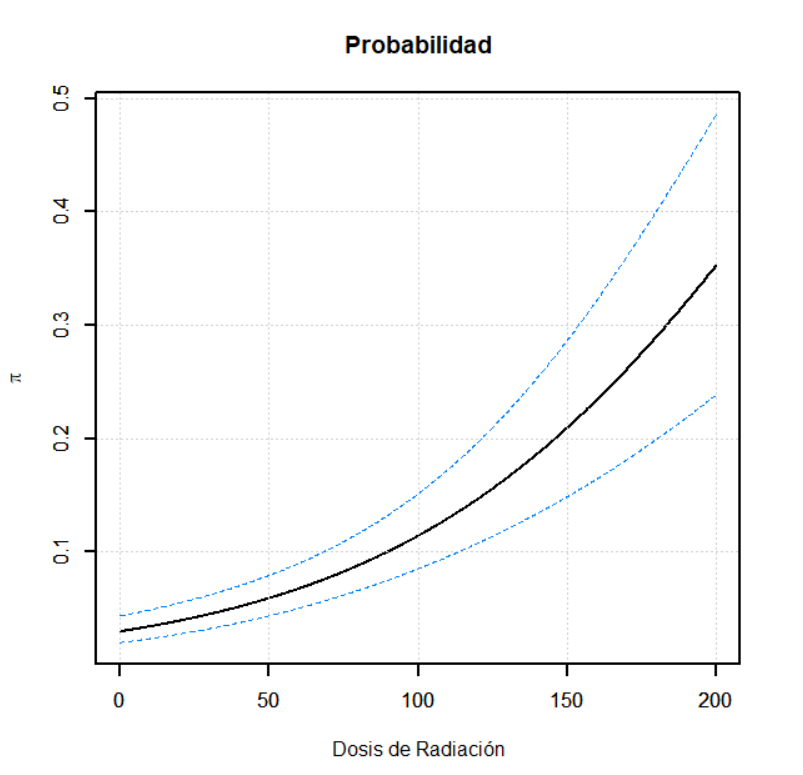
\includegraphics[scale= 0.65]{Im2Ej4.png}
    \caption{Probabilidad de morir por leucemia dado que la causa de muerte fue algún tipo de cáncer, bajo diferentes niveles de exposición a la radiación.}
    \label{fig:nuevanueva}
\end{figure}
  
 
\end{solucion}


\begin{exo}\label{Ej.4}
En la clase vimos el procedimiento iterativo IRLS de estimación de los parámetros de los modelos lineales generalizados, para el modelo de regresión logística.  En este caso, para obtener el algoritmo de estimación, se consideraban las siguientes relaciones: 
\begin{equation*}
    \eta = \ln\pare{\frac{\mu}{1 - \mu}}, \ \frac{\partial \eta}{\partial \mu} = g'(\mu) = \frac{1}{\mu(1 - \mu)} \text{ y } W = n\mu(1 - \mu). 
\end{equation*}
Haga lo siguiente:
\begin{itemize}
    \item[a)] Haga el desarrollo de las relaciones anteriores para el modelo de regresión Poisson.
    \item[b)] Obtenga el algoritmo correspondiente a la regresión Poison.
    \item[c)] En la tabla en la figura \ref{fig:my_label2} se muestran los números de casos de AIDS que se presentaron en los años señalados, en Bélgica a partir de 1981. Se asume que estos datos siguen un modelo de regresión de Poisson, donde la variable explicativa son los años y la respuestas los números de casos por año. 
\end{itemize}
\end{exo} 
\begin{figure}[htb]
    \centering
    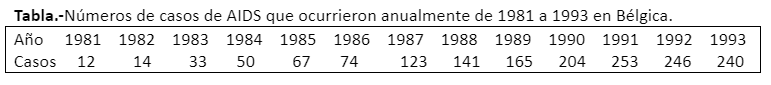
\includegraphics[scale = 0.8]{Im2.png}
    \caption{Datos: Ejercicio 4}
    \label{fig:my_label2}
\end{figure}
\begin{rem}
Para este ejercicio, se considerará una liga Canónica puesto que ninguna función liga ha sido especificada. Además, para este ejercicio tome en cuenta que la notación \(\NN_0\) será utilizada para hacer referencia al conjunto \(\NN \cup \kis{0}.\)
\end{rem}
\begin{solucion}
\noindent\textbf{a)} Inicialmente, considere la función masa de probabilidades de una variable aleatoria Poisson de media \(\mu\): 
\[
p(y | \mu) = \frac{\exp\kis{-\mu}\mu^{y}}{y!}, \ y \in \NN_0, 
\]
y, note que 
\[
 \frac{\mu^{y}}{y!} = \exp\kis{y\log(\mu) - \log(y!)},  \ y \in \NN_0. 
\]
De las igualdades anteriores se concluye que 
\[
p(y | \mu) = \exp\kis{y\log(\mu) - \log(y!) - \mu}, \ y \in \NN_0. 
\]
Así, tome \(\omega = 1, \ \phi = 1, \theta = \log(\mu), \ \mu= b(\theta) = e^{\theta}\) y \(c(y,\phi) = -\log(y!)\) entonces 
\[
p(y|\mu)= p(y|\theta, \phi) = \exp\kis{\frac{y\theta - b(\theta)}{\phi/\omega}+c(y, \phi )},  \ y \in \NN_0. 
\]
Por lo que, se concluye que la distribución Poisson es un miembro de la Familia Exponencial de Dispersión, con: 
\begin{align}
    &\text{Parámetro canónico } \theta = \log(\mu). \label{cano}\\
    &\text{Parámetro de dispersión } \phi = 1. \nonumber\\
    &\text{Función de cumulantes } \mu = b(\theta) = e^{\theta}.\nonumber 
\end{align}
Además, se tiene que 
\begin{equation}\label{LaVariance}
    &V(\mu) = \frac{\partial \mu}{\partial \theta} = \frac{\partial}{\partial \theta}e^{\theta} = e^{\theta} = e^{\ln(\mu)} = \mu. 
\end{equation}
Tome, ahora por \(g:(0, \infty) \to \RR_{+}\) a la liga canónica, la cual por \eqref{cano} esta dada por 
\begin{equation}\label{Lacanonica}
    g(\mu) = \ln(\mu).
\end{equation}
Y suponga que existe un predictor lineal \(\eta\) y covariables \(x_1, \hdots, x_p\) tales que 
\[¨
 g(\mu) = \eta = \beta_{0} + \sum_{j=1}^{p}\beta_{j}x_{j}.  
\]
Entonces 
\begin{equation}\label{deritative}
  \frac{\partial \eta}{\partial \mu} = g'(\mu) = \frac{1}{\mu}.  
\end{equation}

Finalmente:
\[
W = \frac{1}{[g'(\mu)]^2 V(\mu)} = \frac{\mu^2}{\mu} = \mu.
\]

\noindent\textbf{b)} Suponga que tiene \(y_1,\hdots,y_N\) observaciones de conteos, donde \(y_i\) proviene de una distribución Poisson de media \(\mu_i\), \(i \in \kis{1, \hdots, N}\), y suponga que se quiere ajustar un GLM Poisson con liga canónica, utilizando una matriz de covariables \(n\times p\) con \(p < n\), si denota por \(\mathbf{x}_i'\) a la \(i\)-ésima fila de \(X\), entonces el algoritmo IRLS queda dado como: 
\begin{enumerate}
    \item Se inicia con 
    \[
    \hat{\mu}^{0}_i = y_i \text{ y } \eta^{0}_i = g(\hat{\mu}^{0}_i), \ i\in\kis{1,\hdots, N}  
    \]
    En caso, de que la elección realizada cause problemas con la definición de la función liga, se puede añadir una pequeña perturbación a los datos. Por ejemplo, en el caso de conteos Poisson es possible que alguna \(y_i = 0\), lo que implicaría al llevar a cabo el procedimiento anterior, que se este tomando el logaritmo natural de cero o que se este dividiendo entre cero, por ello, una mejor elección será 
    \[
    \hat{\mu}^{0}_i =\begin{cases}
     y_i + 0.1 & \text{ si } y_i=  0,\\ 
     y_i & \text{ si } y_i > 0. 
     \end{cases}\text{ y } \hat{\eta}^{0}_i = g(\hat{\mu}^{0}_i) = \ln(\hat{\mu}^{0}_i), \ i\in \kis{1, \hdots, N}.
    \]
    donde, en la última igualdad se ha utilizado \eqref{Lacanonica}. 
    \item Se calculan los pseudo-datos
    \begin{align*}
    \zeta_{i}^{1} &=\hat{\eta}^{0}_i+ \frac{g'(\hat{\mu^{0}_i})(y_i - \hat{\mu}^{0}_i)}{\alpha(\hat{\mu}^0_i)}\\ 
    &= \ln(\hat{\mu}^{0}_i) + \frac{(y_i - \hat{\mu}^{0}_i)}{\hat{\mu^{0}_i}\alpha(\hat{\mu}^0_i)},  \ i\in \kis{1, \hdots, N},
    \end{align*}
    donde, en la última igualdad se ha utilizado \eqref{deritative}. Y los pesos iterativos 
    \begin{align*}
    w_{i}^{1} &= \frac{\alpha(\hat{\mu}^{0}_i)}{(g'(\hat{\mu}^{0}_i))^2V(\hat{\mu}_i)}=\frac{\alpha(\hat{\mu}^{0}_i)}{(g'(\hat{\mu}^{0}_i))^2V(\hat{\mu}_i)}\\
    &=\alpha(\hat{\mu}^{0}_i)\mu^{0}_i,  \ i\in \kis{1, \hdots, N}.
    \end{align*}
   donde, en la última igualdad se ha utilizado \eqref{deritative} y \eqref{LaVariance}. Cuando, \(\alpha(\mu) = 1\) se le denomina peso de Fischer, y el método anterior coincide con el Scoring de Fischer. 
   \item Encontrar \(\hat{\beta}^1\); que es la solución al problema de mínimos cuadrados ponderados siguiente:
    \[
     \hat{\beta}^{1} = argmin_{\beta}\corch{\sum_{i = 1}^{N}w_i(\zeta_i - \mathbf{x}_i'\beta)^2}. 
    \]
    Luego, se actualizan\footnote{Donde, \(\exp\kis{ \hat{\eta}^{1}}\) debe interpretarse como aplicar la función exponencial a cada entrada del vector \(\hat{\eta^{1}}\).} 
    \[
    \hat{\eta}^{1} = X\hat{\beta}^{1}, \ \hat{\mu}^{1} = g^{-1}\pare{\hat{\eta}^{1}} =\exp\kis{ \hat{\eta}^{1}},   
    \] 
    donde, en la última igualdad se ha utilizado \eqref{Lacanonica}.  
    \item Se calcula la Deviance total con los valores ajustados \(\hat{\mu}^{1} =(\hat{\mu}^{1}_1, \hdots, \hat{\mu}^{1}_N)\):
    \[
    D(y,\hat{\mu}^{1}) = 2\sum_{j = 1}^{n}\kis{y_j \ln(y_j/\hat{\mu}^{1}_j) - (y_j - \hat{\mu}^{1}_j)}.
    \]
    Si:\footnote{El siguiente criterio es usado por el software \(R\) para declarar convergencia del Método. Donde, \(D(y,\hat{\mu}^{0})\) es la Deviance total calculada con los valores ajustados \(\hat{\mu}^{0} =(\hat{\mu}^{0}_1, \hdots, \hat{\mu}^{0}_N)\).}  
    \[
    \frac{\abs{D(y,\hat{\mu}^{1}) - D(y,\hat{\mu}^{0})}}{D(y,\hat{\mu}^{1}) + 0.1} < \ee, 
    \]
    donde \(\ee\) suele ser una cantidad pequeña, empíricamente \(\ee = 10^{-8}\). El algoritmo acaba y la solución es \(\hat{\beta}^{1}\). En caso contrario, se repite con \(\hat{\eta}^{1} = (\hat{\eta}^{1}_1, \hdots, \hat{\eta}^{1}_N)\) y \(\hat{\mu}^{1} =(\hat{\mu}^{1}_1, \hdots, \hat{\mu}^{1}_N)\) todos los pasos realizados desde el paso dos con \(\hat{\eta}^{0} = (\hat{\eta}^{0}_1, \hdots, \hat{\eta}^{0}_N)\) y \(\hat{\mu}^{0} =(\hat{\mu}^{0}_1, \hdots, \hat{\mu}^{0}_N)\). Y así de manera iterativa hasta que la condición de las deviances se cumpla.
\end{enumerate}

\noindent\textbf{c)} Para este inciso se programó en \(R\) el algoritmo anterior, el código puede ser visto en el Script Ejercicio3.R adjunto a este trabajo. De este modo, denote por \(y\) al vector de observaciones de casos de AIDS por año y por \(x\) al vector de datos con los años en que ocurrieron dichos caso, codificados de la siguiente manera \(1981 = 0, \ 1982 = 1, \hdots, \ 1992=11\) y \(  1993 = 12\), se utilizó el procedimiento IRLS programado para estimar los coeficientes del modelo
\begin{equation}\label{conint}
  \ln(\mu_i) = \beta_0 + \beta_1 x_i, \ i\in \kis{1, \hdots, 13},  
\end{equation}
donde \(\mu_i = \EE[y_i | x_i]\). Lo que arrojó los resultados presentados en el Cuadro \ref{tab:ref1}: 
\begin{table}[H]
        \centering
        \begin{tabular}{@{}l@{\hskip 0.3in}r@{\hskip 0.3in}r@{\hskip 0.3in}r@{}}
            \toprule
            Iter&\(\hat{\beta}_0\)  & \(\hat{\beta}_1\)& Deviance Total \\
            \midrule
                1 &3.426& 0.195& 82.491\\ 
                2 &3.345& 0.202& 80.688\\
                3 &3.343& 0.202& 80.686\\ 
                4 &3.343& 0.202& 80.686\\
            \bottomrule
        \end{tabular}
        \caption{Resultados del Procedimiento IRLS, para la estimación de los coeficientes del modelo que considera intercepto.}
        \label{tab:ref1}
\end{table}
En el Cuadro \ref{tab:ref1}, puede observarse que el método convergió después de 4 iteraciones, que las estimaciones de los coeficientes están dadas por 
\[
\hat{\beta}_0 =3.343, \  \hat{\beta}_1 = 0.202, 
\] 
y que la Deviance Residual de este modelo tiene un valor de 
\[
D = 80.686.
\]
Los cálculos anteriores se constataron con la librería \(glm\) de \(R\) arrojando resultados idénticos, además, haciendo uso de dicha librería se obtuvo un \(AIC\), para este modelo de: 
\begin{equation}\label{AIC.Mod1}
AIC  = 166.4.     
\end{equation}
Por otro lado, puesto que la redacción del ejercicio era algo confusa, se decidió ajustar el modelo \eqref{conint} sin considerar el intercepto, es decir: 
\begin{equation}\label{sinint}
  \ln(\mu_i) = \beta_1 x_i, \ i\in \kis{1, \hdots, 13},  
\end{equation}
donde \(\mu_i = \EE[y_i | x_i]\). Y, haciendo uso del método IRLS programado, se obtuvieron los resultados presentados en el Cuadro \ref{tab:ref2} 
\begin{table}[H]
        \centering
        \begin{tabular}{@{}l@{\hskip 0.3in}r@{\hskip 0.3in}r@{}}
            \toprule
            Iter & \(\hat{\beta}_1\)& Deviance Total \\
            \midrule
                   1&  0.5563& 1573.138\\ 
                    2&0.5289& 1394.694 \\
                    3&0.5238& 1390.401 \\
                    4& 0.5236& 1390.398 \\
                    5& 0.5236& 1390.398\\
            \bottomrule
        \end{tabular}
        \caption{Resultados del Procedimiento IRLS, para la estimación de los coeficientes del modelo sin intercepto.}
        \label{tab:ref2}
\end{table}
En el Cuadro \ref{tab:ref2}, puede notar que el método convergió después de 5 iteraciones, que la estimación del coeficiente de pendiente esta dada por 
\[
 \hat{\beta}_1 = 0.5236, 
\] 
y que la Deviance Residual de este modelo tiene un valor de 
\[
D =  1390.398.
\]
Nuevamente, los cálculos anteriores se compararon con los obtenidos haciendo uso de la librería \(glm\) de \(R\), lo que corroboró los cálculos obtenidos, además, ocupando dicha librería se obtuvo un \(AIC\) para este modelo de: 
\begin{equation*}
AIC  =  1474.     
\end{equation*}
Los \(AIC\) se calcularon para comparar los modelos expuestos. En este caso, resulta evidente que el modelo en \eqref{conint} posee un mejor ajuste, al ver que el AIC del modelo \eqref{sinint} es de \( 1474\), lo cual es mucho mayor que el \(AIC\) del modelo \eqref{conint} presentado en \eqref{AIC.Mod1}. 
\end{solucion}

\begin{exo}\label{Ej.5}
En un estudio médico se cuentan los números de pólipos en pacientes que padecen poliposis adenomatosa familiar, después de recibir un tratamiento con un nuevo medicamento, o de un placebo. En la Tabla en la figura \ref{fig:my_label3} se presentan los datos asociados al estudio.
Haga lo siguiente
\begin{itemize}
    \item[a)] Grafique los datos y coméntelos.
    \item[b)] Encuentre un modelo MLG Poisson adecuado para modelar los datos y justifique que hay sobredispersion.
    \item[c)] Ajuste un modelo cuasi-Poisson a los datos.
    \item[d)] Ajuste un MLG binomial negativo a los datos. 
    \item[e)] Elija un modelo final y comente su elección.
\end{itemize}
\end{exo} 
\begin{figure}[htb]
    \centering
    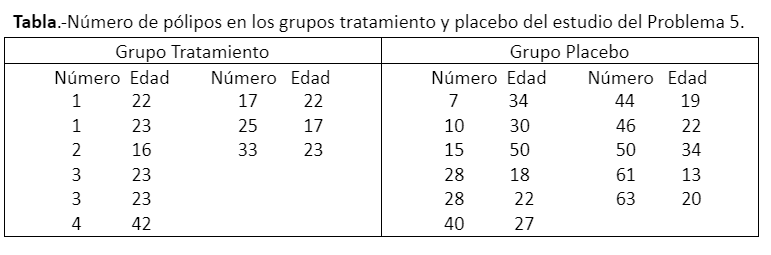
\includegraphics[scale = 0.8]{Im3.png}
    \caption{Datos ejercicio 5.}
    \label{fig:my_label3}
\end{figure}
\begin{solucion}

\end{solucion}


\nocite{dunn_generalized_2018}
\printbibliography

\end{document}
